\section{Introduction}

\noindent Level-1 trigger (L1) is the first stage of CMS triggering system. This is a purely hardware stage during which LHC data rate is currently reduced from 20MHz to 100kHz within a latency of $6.4~\mu s$. Because of this very short latency, only the calorimeters and the muon subdetectors are part of L1 for the moment. The tracking detectors are used only at the second stage, knwon as the High-Level Trigger (HLT). 

\noindent Fig.~\ref{fig:L1Rates} illustrates how the lack of tracking at L1 might affect trigger efficiency. This figure shows, at LHC nominal luminosity, the rates of muons as a function of $p_T$. The line shows the generated muon rate, while black stars and red dots show muon rates after HLT and L1 respectively. The L1 muon rate, obtained using only the muon spectrometer, is much higher than the generated rate. It means that a lot of fake muons pass this trigger. These fakes are then cleaned at the HLT, as tracker info provides a much better sensitivity to muon identification than coarse muon info.
 
\begin{figure}[ht!]
\begin{minipage}[t]{7.5cm}
\centering
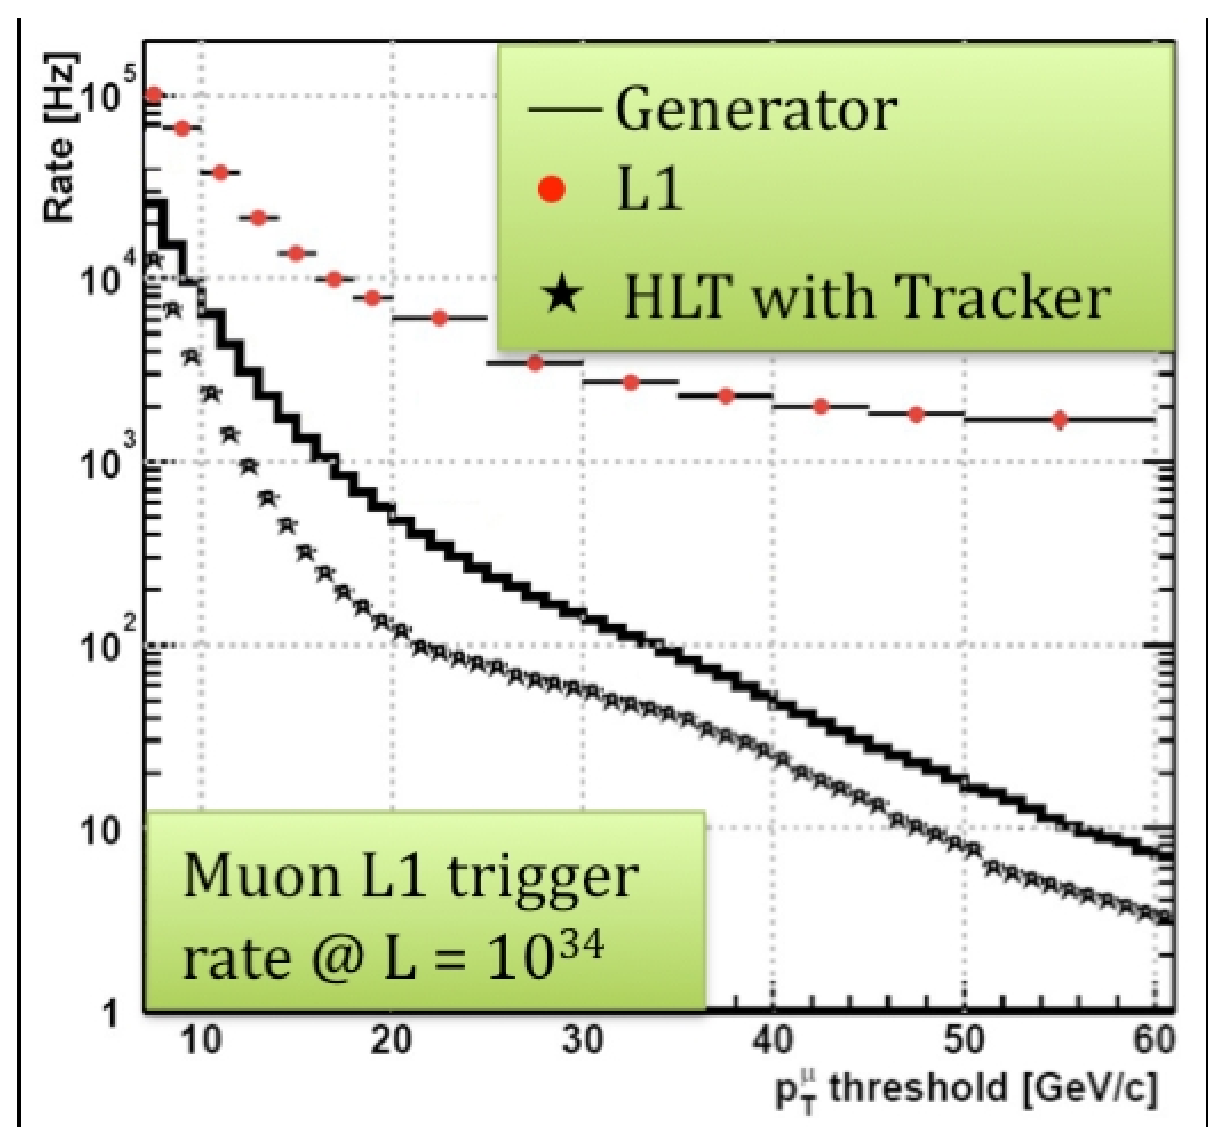
\includegraphics[width=0.99\textwidth]{Plots/CurrentTracker.eps}
\caption{Expected Level-1 single muon rate as a function of $p_{T}$ threshold for a luminosity of $10^{34}cm^{-2}s^{-1}$, in the present system.~\cite{bib:Abb-11}}
\label{fig:L1Rates}
\end{minipage}
\hfill
\begin{minipage}[t]{7.5cm}
\centering
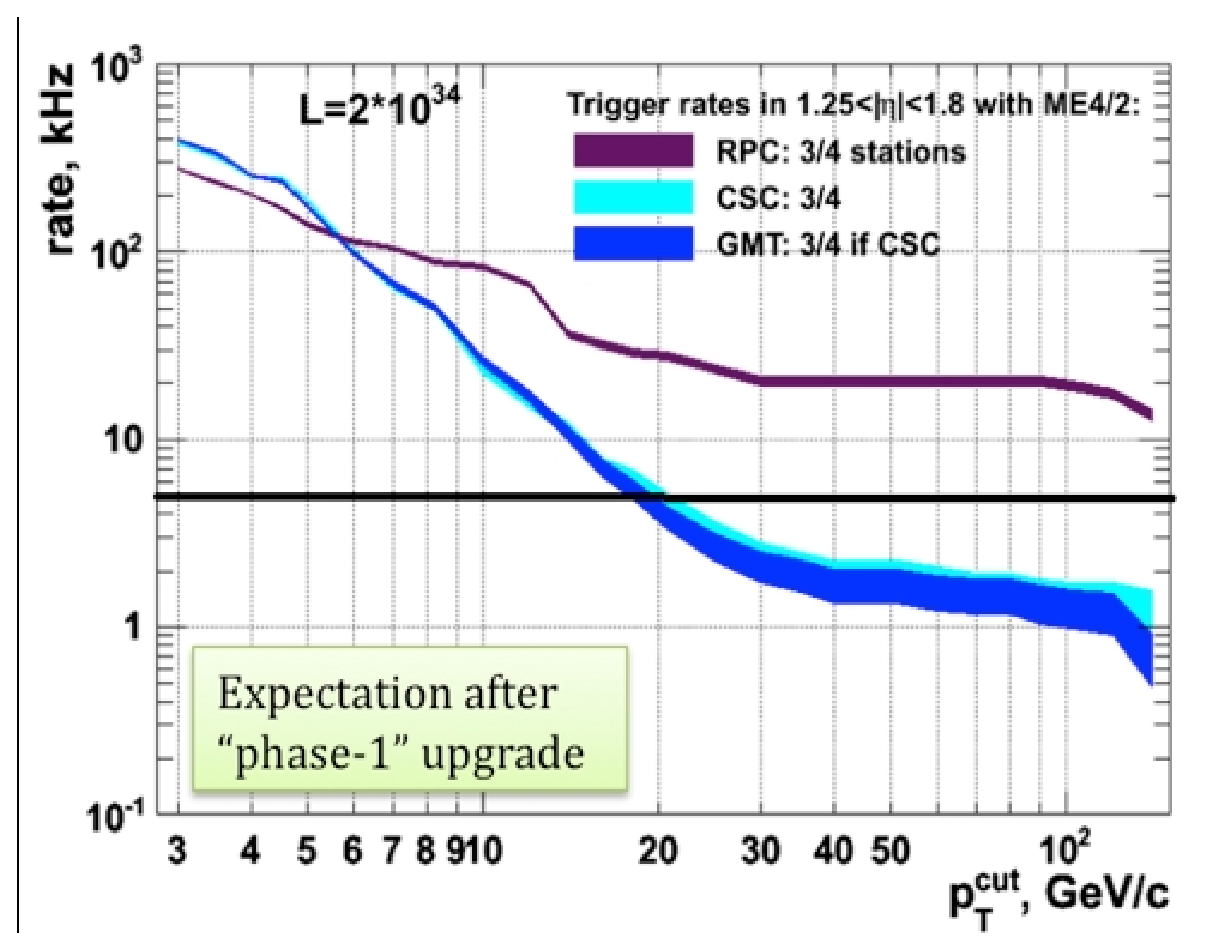
\includegraphics[width=0.99\textwidth]{Plots/21034_tracker.eps}
\caption{Expected threshold after phase 1 trigger upgrade, for a luminosity of $2\times 10^{34}cm^{-2}s^{-1}$.~\cite{bib:Abb-11}}
\label{fig:L1RatesPhase1}
\end{minipage}
\end{figure} 

\noindent One can also see on Fig.~\ref{fig:L1Rates} that fake proportion increases w.r.t. the $p_T$. This is due to the fact that L1 muon system uses coarse resolution information. Therefore high-$p_T$ tracks becomes compatible with straight lines at a certain point, and consequently the L1 muon rate reaches a plateau at high-$p_T$. At $10^{34}cm^{-2}s^{-1}$, this plateau lies at around $1~kHz$. Considering that overall L1 rate is $100~kHz$, the poor discrimination power at high-$p_T$ is not critical.

\noindent However, the plateau level is strongly depending on the instantaneous luminosity. Fig.~\ref{fig:L1RatesPhase1} shows its evolution, for the different muon subdetectors, at $2\times 10^{34}cm^{-2}s^{-1}$. For the RPC, the plateau lies at $20~kHz$, 20\% of the total L1 bandwidth. This is clearly not sustainable anymore. When going to HL-LHC luminosity, the other muons subdetectors also become problematic. In other words, muon indentification is not possible anymore. From there two solutions can be envisaged: increasing the L1 rate or including the tracking at L1. This note is dedicated to the second point.  


\clearpage
